% !TeX spellcheck = en_US

\chapter{Results}
For this project we have chosen to use C++17 and to implement a multi-threaded program to achieve a better execution time upon the computational process using OpenMP, an open standard for parallelism for C, C++ and Fortran programs. The whole execution has been run on a cluster of $10$ \texttt{Intel(R) Xeon(R) CPU E5430 @ 2.66GHz - 16GB RAM}. With this computational power, we have been able to perform multiple experiments by varying the $K$-fold value in the cross-validation: $2$, $3$, $5$, $10$, $20$, $50$, $150$, $300$, $750$ during a period of seven days of computation.\\
The program has been written to print all the results in a \texttt{.json} file to achieve an easier data analysis through Python. In all of the experiments, both AdaBoost and Bagging have been trained over the whole data-set with the same hyper-parameter $T$ for each iteration.\\
\begin{figure}[htpb]
	\centering
		\begin{tabular}{c c}
			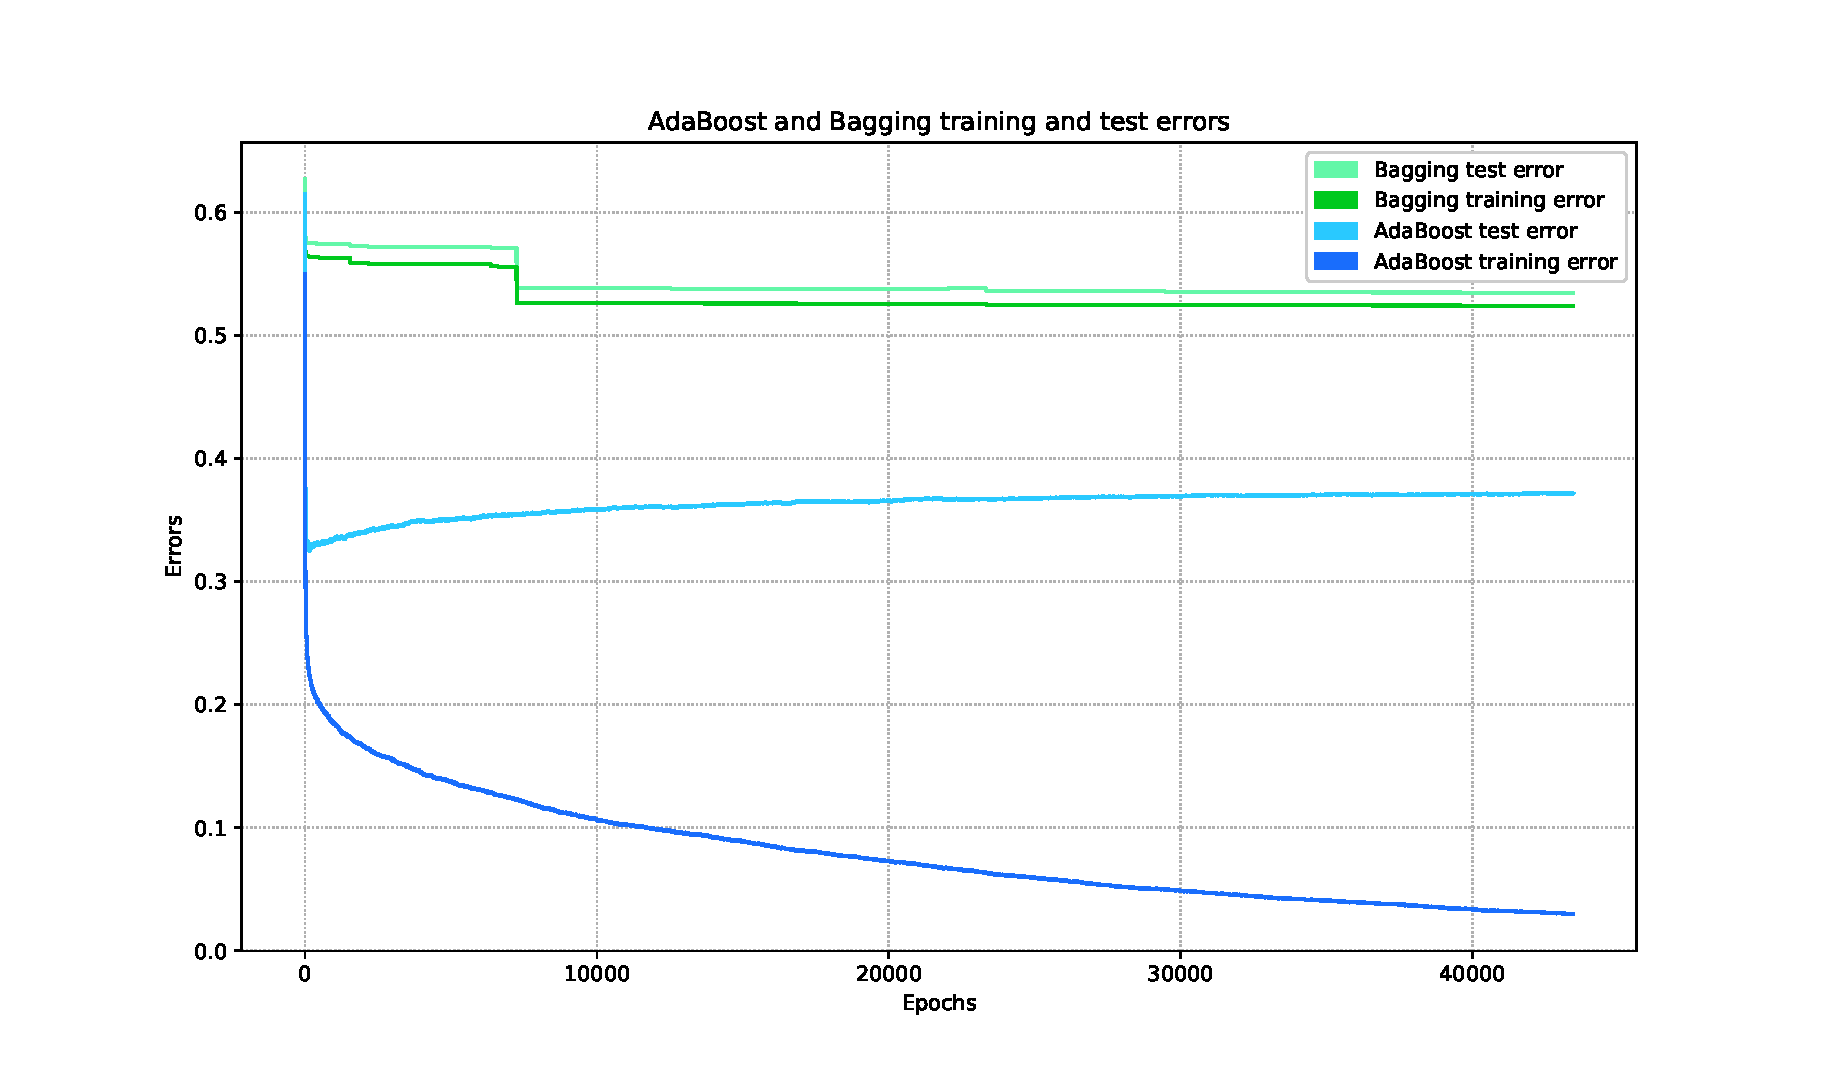
\includegraphics[scale=0.2]{figs/report_k2.eps} & 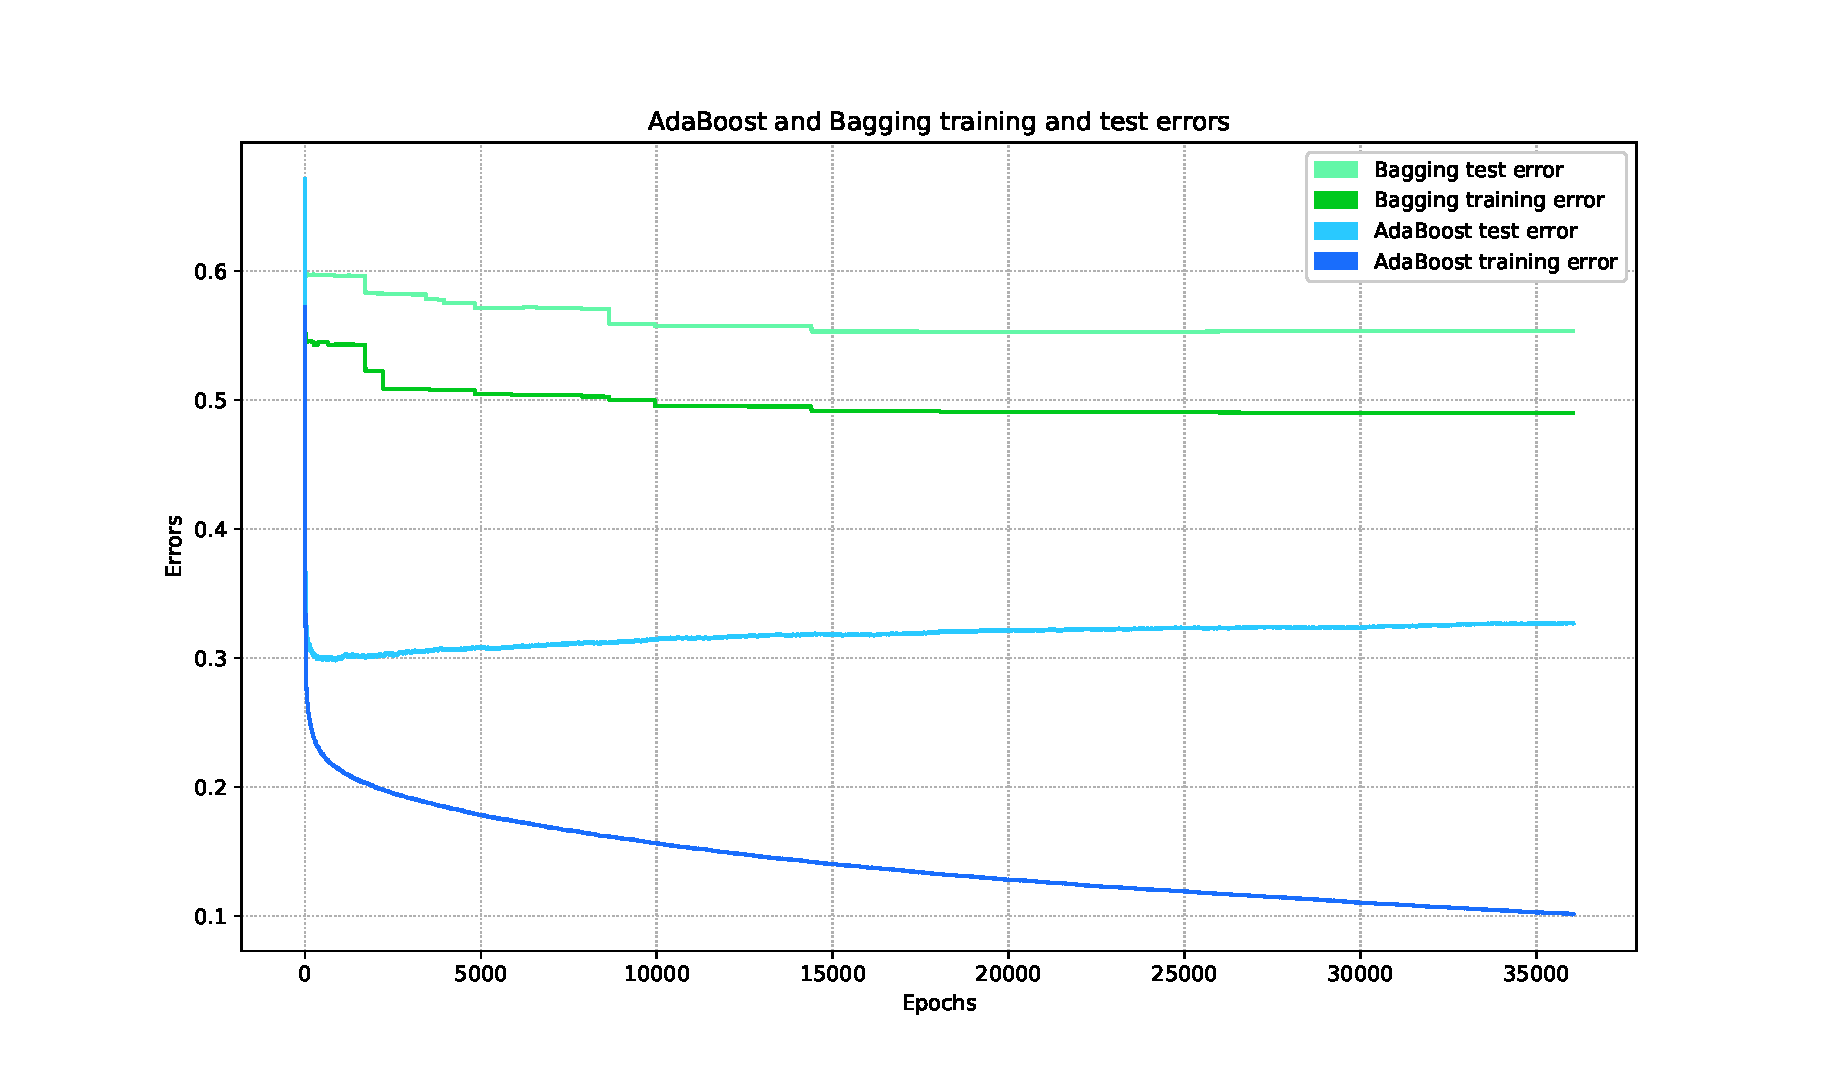
\includegraphics[scale=0.2]{figs/report_k5.eps} \\
			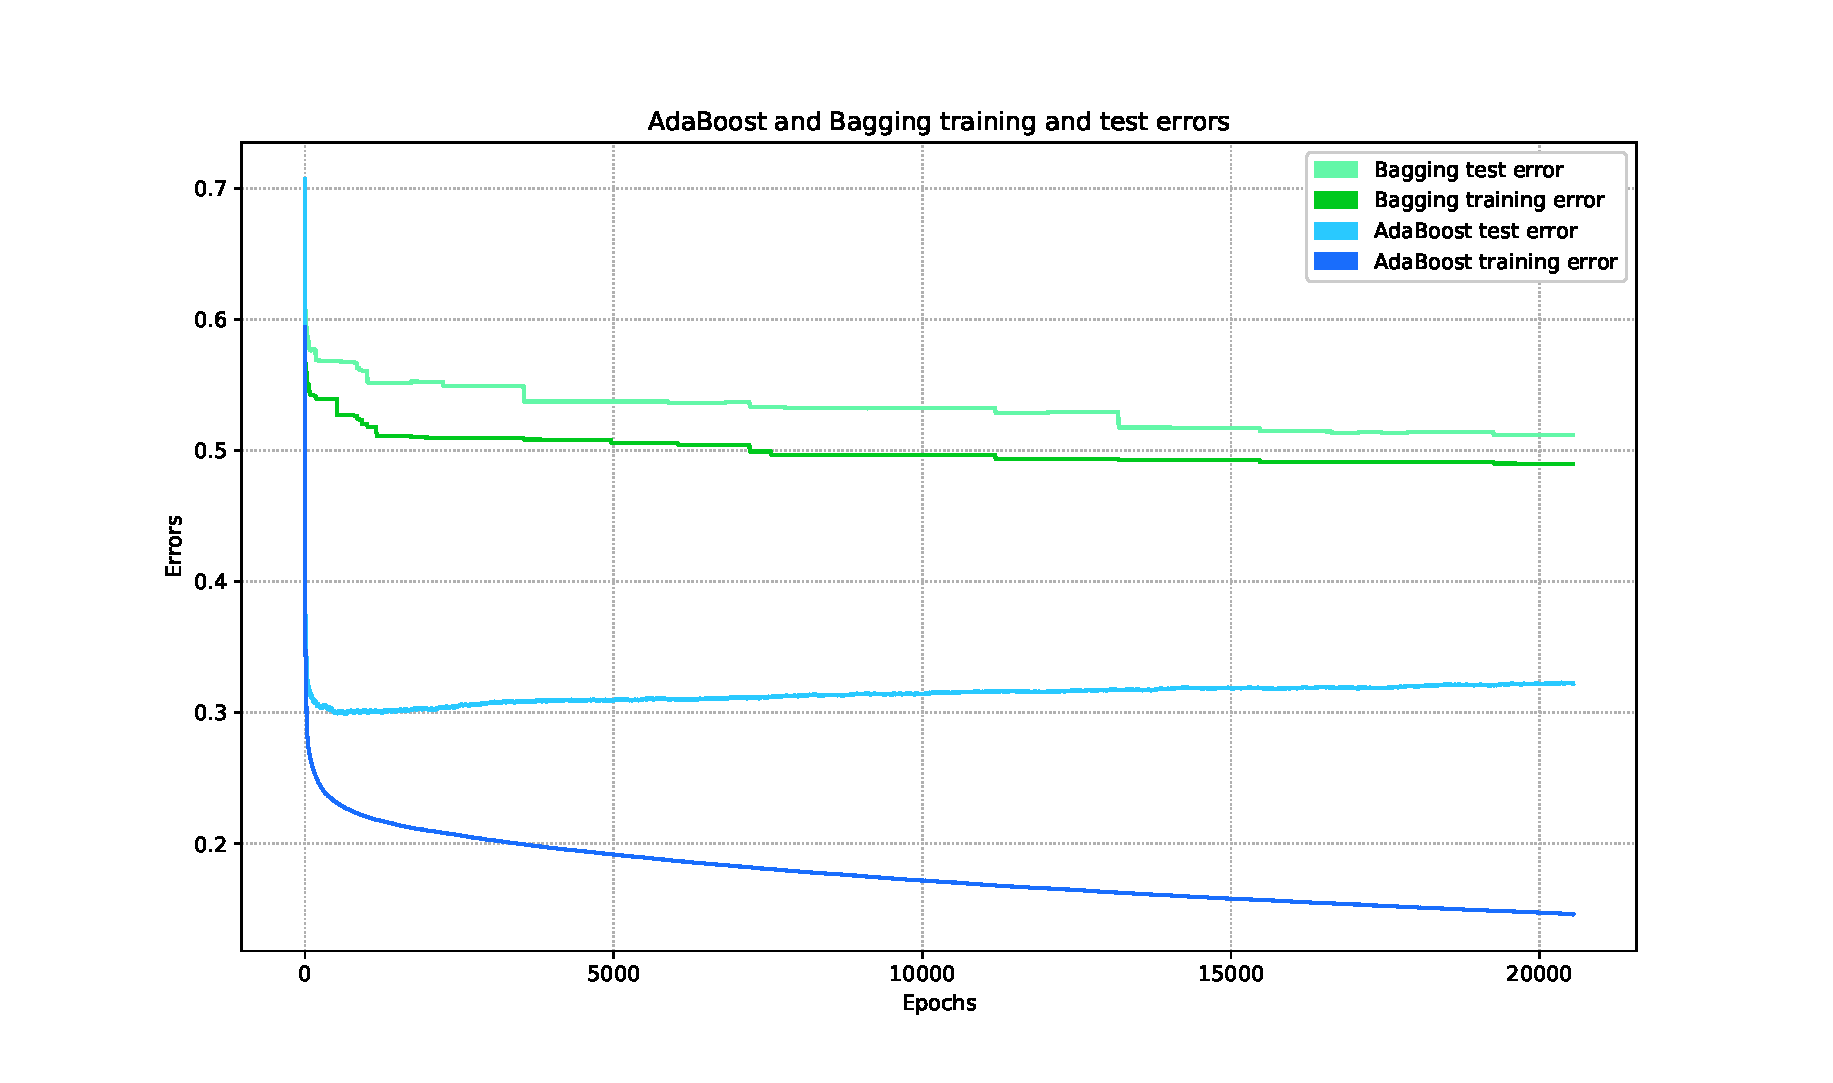
\includegraphics[scale=0.2]{figs/report_k20.eps} &
			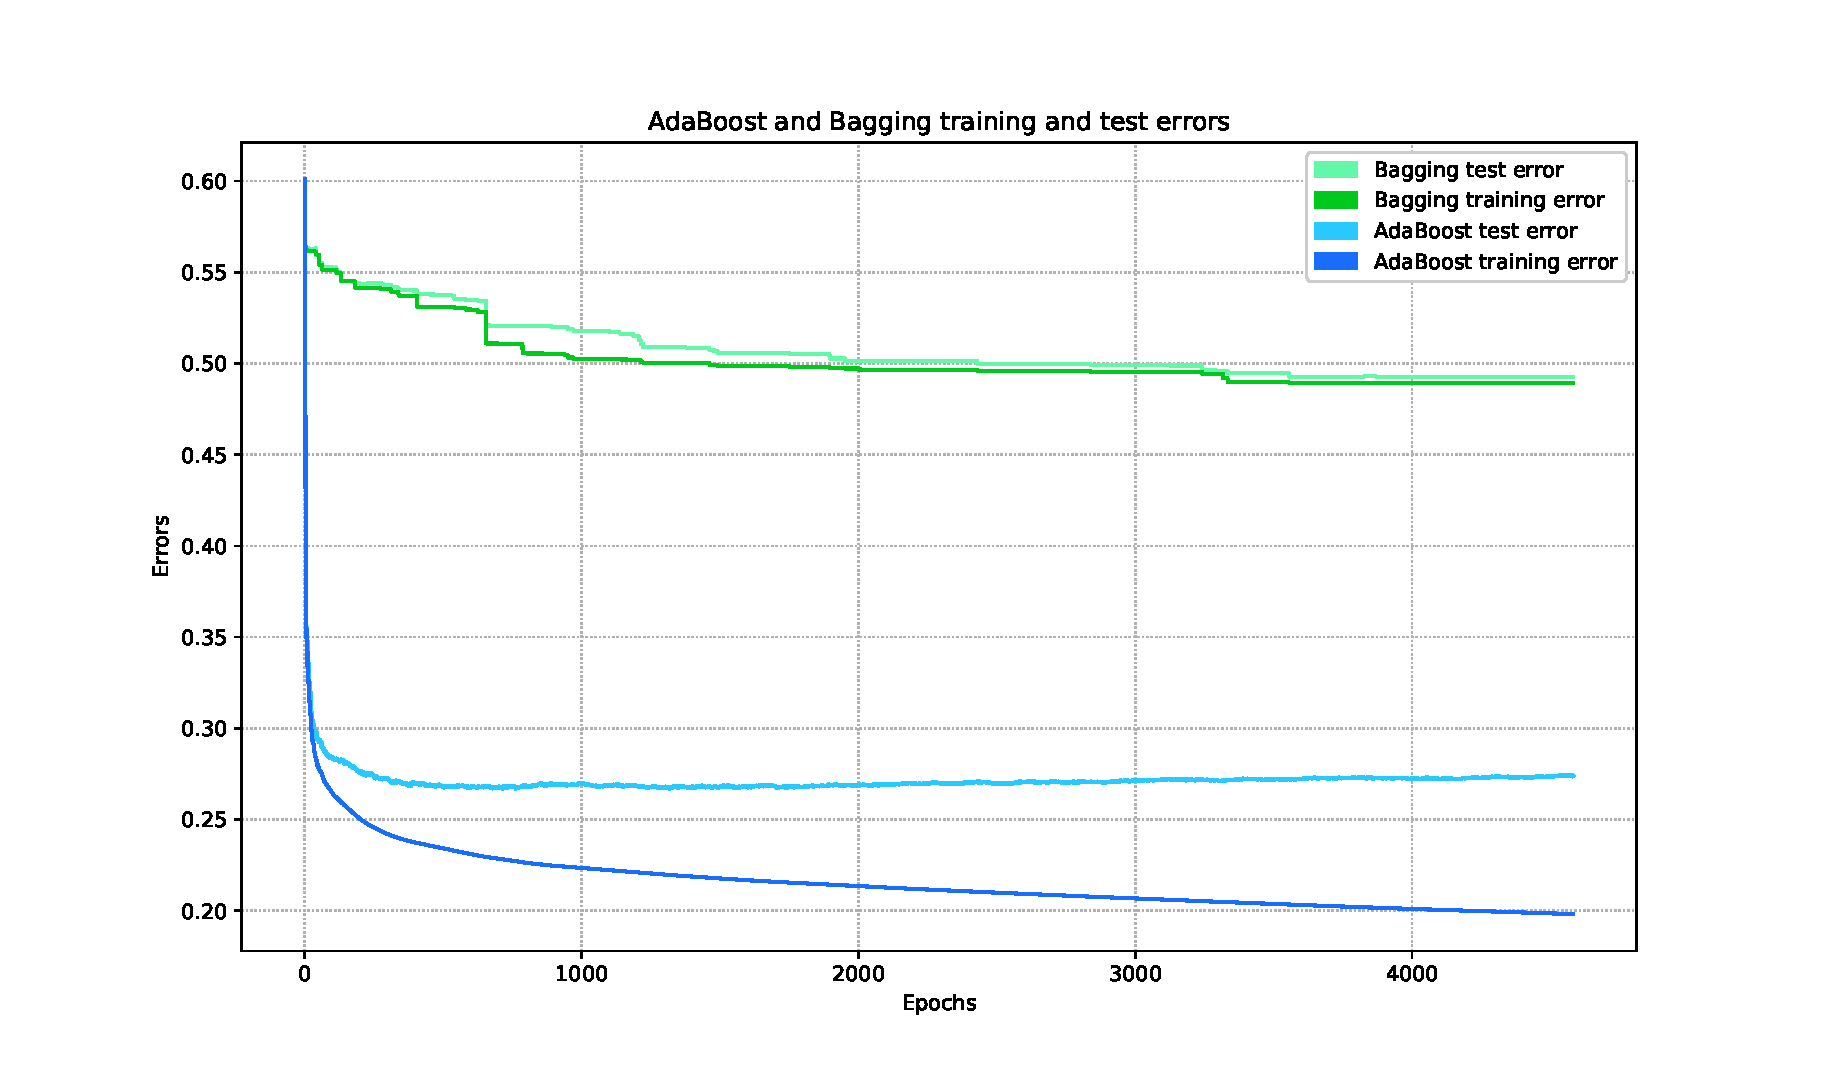
\includegraphics[scale=0.2]{figs/report_k750.eps} \\
		\end{tabular}
\end{figure}
As you can see in \autoref{fig:k20}, AdaBoost is way better than Bagging and it's already possible to catch the best value for $T$, which in this case is $650$ with a test error of $0.29861$.\\
Table \autoref{tab:results} summarize all the results for all the $K$-fold experiments.

\begin{table}
\centering
\begin{tabular}{|c|c|c|}
	\hline
	K & Best T value & Test Error \\
	\hline
	2 & 144 & 0.325198412698413 \\
	\hline
	3 & 260 & 0.308068783068783 \\
	\hline
	5 & 873 & 0.298148148148148 \\
	\hline
	10 & 673 & 0.302050264550265 \\
	\hline
	20 & 650 & 0.29861 \\
	\hline
	50 & 998 & 0.291995716127904 \\
	\hline
	150 & 637 & 0.281324092409241 \\
	\hline
	300 & 563 & 0.272647058823529 \\
	\hline
	750 & 714 & 0.26634920634921 \\
	\hline
\end{tabular}
\caption{All the results varying the parameter $K$ in the cross-validation}
\label{tab:results}
\end{table}
